% Generated by `uv run analyze`; needs \usepackage{pgfplots}
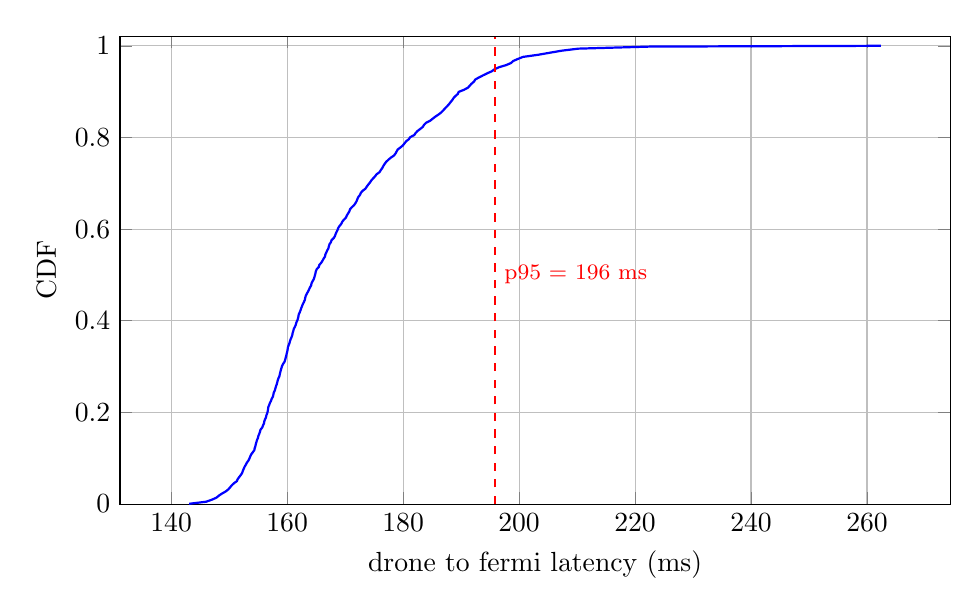
\begin{tikzpicture}
\begin{axis}[xlabel={drone to fermi latency (ms)}, ylabel={CDF}, width=\columnwidth, height=0.62\columnwidth, grid=major, ymin=0, ymax=1.02]
\addplot[thick, blue] coordinates {(143.106,0.0006) (146.039,0.0051) (147.044,0.0096) (147.822,0.0140) (148.244,0.0185) (148.785,0.0230) (149.414,0.0275) (149.867,0.0320) (150.169,0.0365) (150.47,0.0410) (150.846,0.0455) (151.334,0.0500) (151.484,0.0545) (151.744,0.0590) (152.02,0.0635) (152.247,0.0680) (152.371,0.0725) (152.52,0.0770) (152.673,0.0815) (152.887,0.0860) (153.058,0.0904) (153.327,0.0949) (153.505,0.0994) (153.644,0.1039) (153.81,0.1084) (154.076,0.1129) (154.34,0.1174) (154.409,0.1219) (154.528,0.1264) (154.609,0.1309) (154.71,0.1354) (154.816,0.1399) (154.98,0.1444) (155.048,0.1489) (155.206,0.1534) (155.33,0.1579) (155.417,0.1624) (155.705,0.1669) (155.838,0.1713) (156.005,0.1758) (156.061,0.1803) (156.195,0.1848) (156.354,0.1893) (156.429,0.1938) (156.575,0.1983) (156.661,0.2028) (156.713,0.2073) (156.766,0.2118) (156.91,0.2163) (157.038,0.2208) (157.225,0.2253) (157.346,0.2298) (157.546,0.2343) (157.632,0.2388) (157.705,0.2433) (157.883,0.2478) (157.975,0.2522) (158.073,0.2567) (158.209,0.2612) (158.302,0.2657) (158.388,0.2702) (158.518,0.2747) (158.678,0.2792) (158.745,0.2837) (158.835,0.2882) (158.926,0.2927) (159.031,0.2972) (159.14,0.3017) (159.324,0.3062) (159.566,0.3107) (159.671,0.3152) (159.763,0.3197) (159.864,0.3242) (159.933,0.3287) (160.031,0.3331) (160.089,0.3376) (160.136,0.3421) (160.262,0.3466) (160.408,0.3511) (160.497,0.3556) (160.611,0.3601) (160.78,0.3646) (160.9,0.3691) (160.96,0.3736) (161.076,0.3781) (161.164,0.3826) (161.356,0.3871) (161.503,0.3916) (161.596,0.3961) (161.759,0.4006) (161.874,0.4051) (161.951,0.4096) (162.011,0.4140) (162.185,0.4185) (162.317,0.4230) (162.434,0.4275) (162.58,0.4320) (162.715,0.4365) (162.899,0.4410) (163.055,0.4455) (163.124,0.4500) (163.221,0.4545) (163.401,0.4590) (163.598,0.4635) (163.772,0.4680) (163.93,0.4725) (164.145,0.4770) (164.204,0.4815) (164.385,0.4860) (164.577,0.4904) (164.702,0.4949) (164.8,0.4994) (164.895,0.5039) (164.964,0.5084) (165.126,0.5129) (165.466,0.5174) (165.558,0.5219) (165.876,0.5264) (166.099,0.5309) (166.283,0.5354) (166.528,0.5399) (166.594,0.5444) (166.757,0.5489) (166.918,0.5534) (167.113,0.5579) (167.201,0.5624) (167.305,0.5669) (167.544,0.5713) (167.67,0.5758) (168.031,0.5803) (168.245,0.5848) (168.37,0.5893) (168.523,0.5938) (168.702,0.5983) (168.83,0.6028) (169.067,0.6073) (169.361,0.6118) (169.519,0.6163) (169.816,0.6208) (170.16,0.6253) (170.297,0.6298) (170.524,0.6343) (170.737,0.6388) (170.849,0.6433) (171.165,0.6478) (171.54,0.6522) (171.79,0.6567) (171.99,0.6612) (172.12,0.6657) (172.289,0.6702) (172.572,0.6747) (172.715,0.6792) (173.027,0.6837) (173.51,0.6882) (173.734,0.6927) (174.002,0.6972) (174.282,0.7017) (174.52,0.7062) (174.837,0.7107) (175.172,0.7152) (175.429,0.7197) (175.935,0.7242) (176.151,0.7287) (176.4,0.7331) (176.59,0.7376) (176.806,0.7421) (177.071,0.7466) (177.439,0.7511) (177.854,0.7556) (178.385,0.7601) (178.674,0.7646) (178.871,0.7691) (179.06,0.7736) (179.535,0.7781) (179.966,0.7826) (180.24,0.7871) (180.522,0.7916) (180.978,0.7961) (181.215,0.8006) (181.914,0.8051) (182.151,0.8096) (182.482,0.8140) (182.946,0.8185) (183.395,0.8230) (183.612,0.8275) (183.965,0.8320) (184.661,0.8365) (185.116,0.8410) (185.566,0.8455) (186.11,0.8500) (186.561,0.8545) (186.914,0.8590) (187.234,0.8635) (187.583,0.8680) (187.907,0.8725) (188.183,0.8770) (188.476,0.8815) (188.699,0.8860) (189.027,0.8904) (189.436,0.8949) (189.586,0.8994) (190.475,0.9039) (191.164,0.9084) (191.488,0.9129) (191.813,0.9174) (192.23,0.9219) (192.444,0.9264) (193.067,0.9309) (193.77,0.9354) (194.486,0.9399) (195.294,0.9444) (195.773,0.9489) (196.573,0.9534) (197.771,0.9579) (198.598,0.9624) (198.995,0.9669) (199.786,0.9713) (200.676,0.9758) (203.232,0.9803) (205.266,0.9848) (207.326,0.9893) (210.211,0.9938) (222.527,0.9983) (262.408,1.0000)};
\draw[red, dashed, thick] (axis cs:195.8,0) -- (axis cs:195.8,1.02);
\node[red, anchor=west, font=\footnotesize] at (axis cs:195.8,0.5) {p95 = 196 ms};
\end{axis}
\end{tikzpicture}
